\documentclass{../indiv}
\graphicspath{{../../images/part1/ch2/}}
\setcounter{chapter}{1}

\begin{document}
	\chapter{初始環境設定}
	\section{\LaTeX 的運作模式與編譯流程}
	先前提到\LaTeX 是一套功能強大且複雜的排版「系統」,顧名思義可知它並非一個獨立運行的程式,而是將每個獨立的小程式串成一組「編譯鍊」(Compile Chain),才得以支援這麼多自動化的功能。
	\begin{figure}[H]
		\centering
		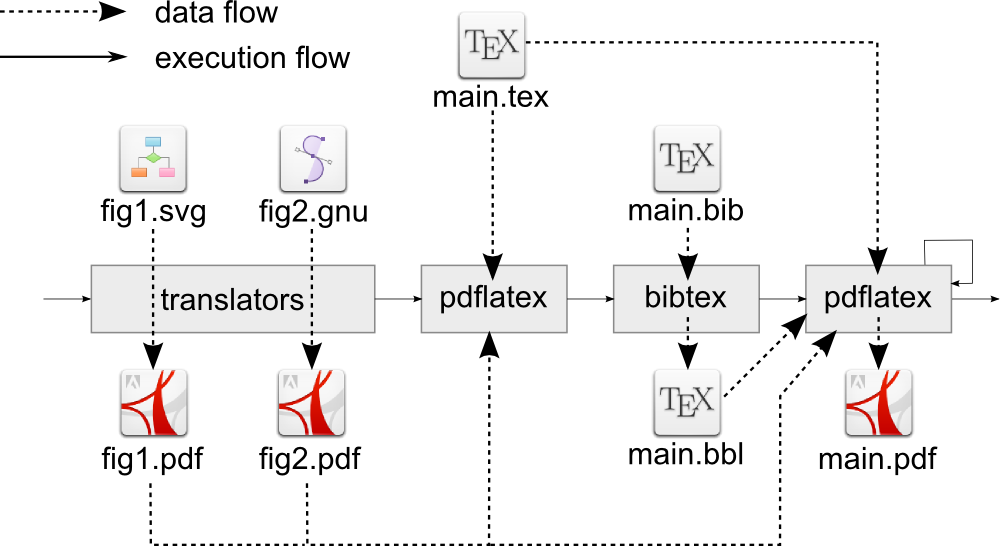
\includegraphics[width=0.6\linewidth]{process.png}
		\caption{一種典型的\LaTeX 文件編譯流程}
		\label{fig:Compile Process}
	\end{figure}
	一份文件的產出還必須仰賴許多字形檔、格式檔與額外的套件包,而套件包之間的相依性也往往非常複雜,不同的文件還可能會用到不同的編譯流程。因此,這些工具不可能讓我們一個一個安裝,因為保證還沒裝完你就會先累死。
	
	幸運的是,科技就是為了便利而存在。網路上早已有很多大佬設計的\TeX /\LaTeX 發行版(Disturbution),裡面就包含了那些最常用的工具,免去手動安裝的煩惱。而且它還有另一個最重要的功能,也就是會自動管理需要用到的套件,缺了什麼就幫你下載什麼,根本就是最偉大的發明之一了{\OSfamily(XD)}。(真不愧是號稱系統管理者的救世主)
	\begin{extra}
		\item 其實許多大型程式的開發也同樣必須透過一連串的工具達成,例如一套典型的開發環境可能會包含:文字編輯器、編譯器、連結器、函式庫、偵錯工具、效能分析工具等等。
		\item 只要是多少聽過或用過Linux的人,也一定對發行版與套件包管理工具的概念不陌生。Python中的\texttt{pip}或\texttt{conda}也是一種套件包管理工具的範例。
	\end{extra}

	\section{安裝\LaTeX 發行版 \textemdash\ \hologo{MiKTeX}}
	貓貓在本書中皆使用Windows作業系統作為示範,而支援Windows的發行版主要有\hologo{MiKTeX}與\TeX\ Live。其實因為各發行版的功能差異很小,再加上貓貓懶得比較兩者的差異,所以就選擇最多人用的\hologo{MiKTeX}作為示範吧 ...
	\begin{table}[H]
		\centering
		\rowcolors{2}{gray!20}{gray!10}
		\OSfamily
		\setlength{\tabcolsep}{10pt}
		\begin{tabular}{T >{\ttfamily\large}p{2.5em} p{7.3cm} p{6.5cm} T}
			\Thline
			\rowcolor{cyan!40} \textrm{\textbf{\large 步驟}} & \textbf{\large 圖示} & \textbf{\large 說明} \\ \Thline
			1. &
			\begin{tabmp}[-0.2]
				\centering
				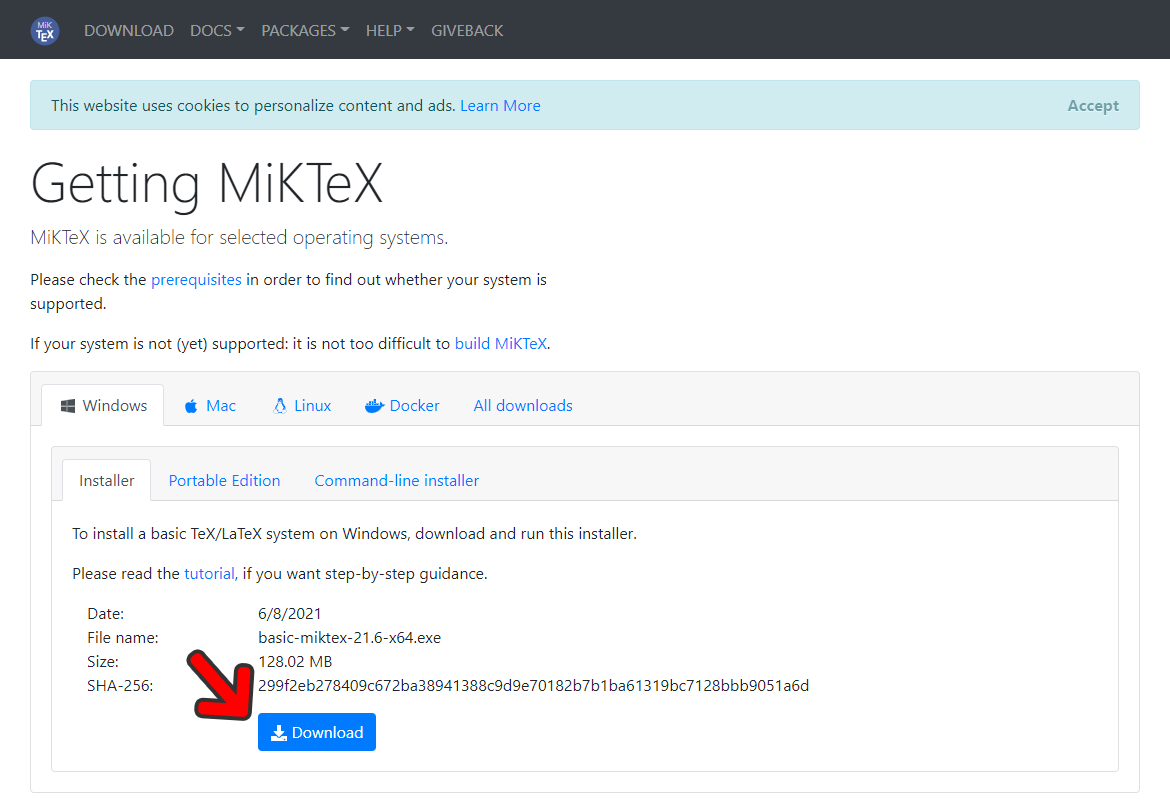
\includegraphics[width=\linewidth]{miktex-install-1.png}
			\end{tabmp} &
			至 \href{https://miktex.org/download}{\hologo{MiKTeX}官方網站} 下載最新的 \hologo{MiKTeX}發行版。\newline 以Windows系統為例,檔名應為\texttt{basic-miktex-(版本)-x64.exe}。\\
			2. &
			\begin{tabmp}[-0.2]
				\centering
				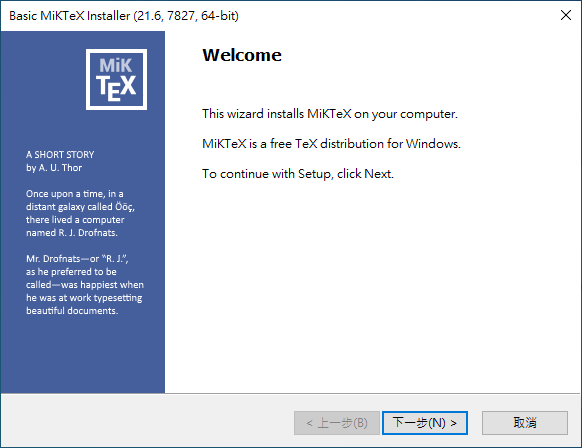
\includegraphics[width=0.49\linewidth]{miktex-install-2.png}
				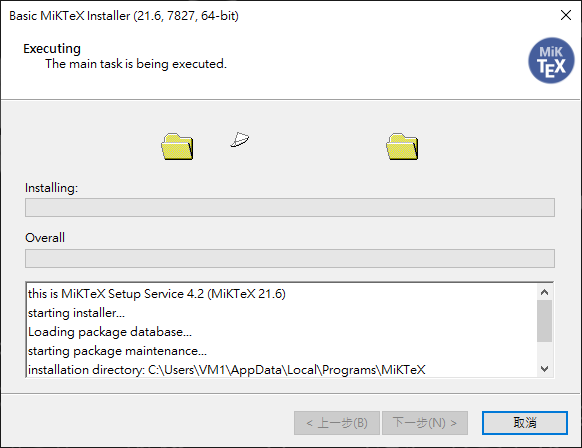
\includegraphics[width=0.49\linewidth]{miktex-install-3.png}\\[1.5mm]
				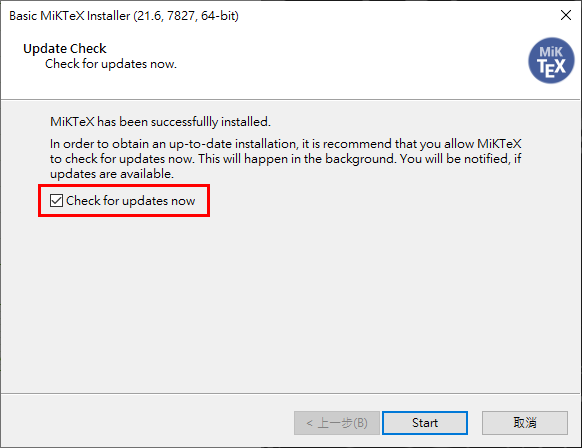
\includegraphics[width=0.49\linewidth]{miktex-install-4.png}
				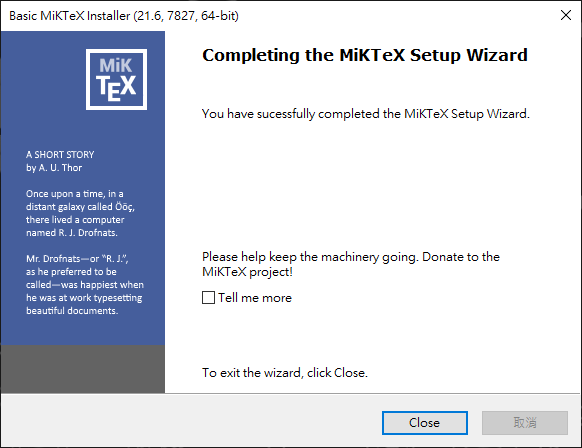
\includegraphics[width=0.49\linewidth]{miktex-install-5.png}
			\end{tabmp} &
			執行安裝程式,之後就是熟悉的連點下一步(XD),並等待安裝程式複製完所有檔案。(預設的設定應該能符合大多數人的需求啦)\newline
			複製完檔案後,記得將{\fontspec{Segoe UI Symbol}\char"2611} Check for updates now打勾,讓套件管理工具檢查是否有套件更新。接著就可以一直下一步,直到安裝程式結束。\\
			3. &
			\begin{tabmp}[-0.3]
				\centering
				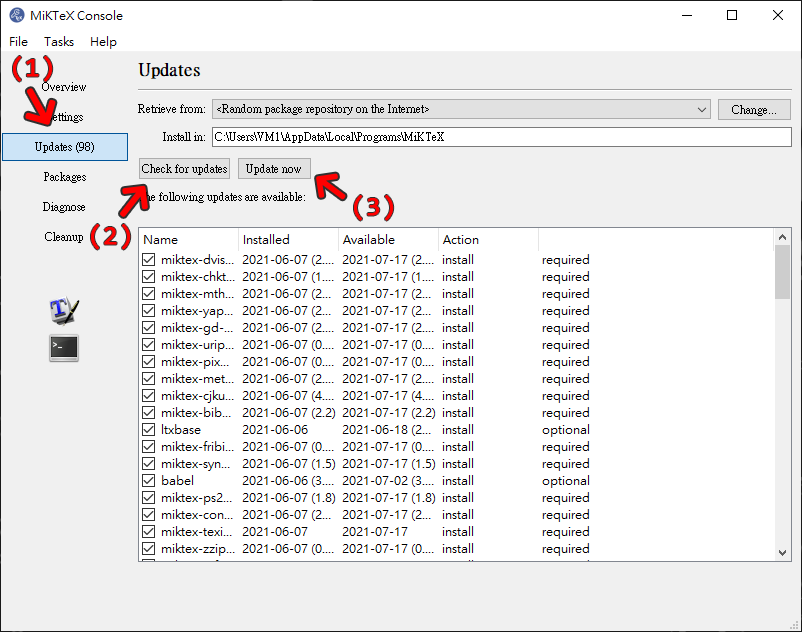
\includegraphics[width=\linewidth]{miktex-install-6.png}
			\end{tabmp} &
			\begin{tabmp}
				\begin{enumerate}[label=\texttt{(\arabic*)}, nosep, left=0pt, labelsep=0.5ex]
					\item 開啟MiKTeX Console,並點擊左側的Updates。
					\item 若下面的列表為空的(或是為了保險起見),點擊Check for updates。
					\item 等待程式檢查更新後,點擊Update now,並更新所有可更新的套件。
				\end{enumerate}
			\end{tabmp}
			\\ \Thline
		\end{tabular}
		\label{tab:MiKTeX Installation}
	\end{table}
	
	\section{安裝套件 \textemdash\ xeCJK}
	
	\section{安裝\LaTeX 編輯器 \textemdash\ Texmaker}
	
	\section{設定Texmaker}
	在此筆者使用\hologo{XeLaTeX}作為編譯引擎,因為他對多國語言的支援度相當廣泛,也是所有引擎中對中文支援最好的引擎之一。
\end{document}